\hrefsection{tsfi.ls.wan}{\tsfisectionname{ls.wan}}

In diesem Abschnitt werden die Protokolle beschrieben, die der TOE über seine
Schnittstelle \lswan{} abwickelt. \tableref{tab:ls.wan.protocols-ports} listet
diese Protokolle und die dafür verwendeten Portnummern.
\figureref{fig:tsfi.ls.wan.protocols} stellt die Protokolle dar, welche die
sicherheitsrelevanten Aspekte des TSFI ausmachen (vgl. die einleitende Bemerkung
zu \chapterref{tsfi.ls}).

\afterpage{%
  \clearpage% Flush earlier floats (otherwise order might not be correct)
  \begin{landscape}% Landscape page
    \centering % Center table
    {
      \label{tab:ls.wan.protocols-ports}
\begin{longtable}{@{}lcllcclp{6cm}@{}}
  \toprule
  Dienst & In/Out & Protokoll & via & Quellport & Zielport & TSFI & Anmerkung \\ \midrule \endhead
  \bottomrule \caption*{Übersicht der Protokoll- und Portnummern für IP/TCP/UDP auf \formatintf{LS.WAN}} \endfoot
  \bottomrule \caption{Übersicht der Protokoll- und Portnummern für IP/TCP/UDP auf \formatintf{LS.WAN}} \endlastfoot
  Basisprotokolle & -- & IEEE802.3 &  -- & -- & -- &    \tsfilink{ls.wan.ether} \\
  & -- & IPv4 & IEEE802.3 & -- & -- &    \tsfilink{ls.wan.ip} \\
  & -- & TCP &  IPv4 & -- & -- &    \tsfilink{ls.wan.tcp} \\
  & -- & UDP &  IPv4 & -- & -- &    \tsfilink{ls.wan.udp} \\[2ex]
  IPSec & Out & IKEv2 & UDP & dyn. & 500 & \tsfilink{ls.wan.ipsec} \\
  & Out & IKEv2 & UDP & dyn. & 4500 & \tsfilink{ls.wan.ipsec} & bei UDP-Encapsulation\\
  & -- & ESP & IPv4 & -- & -- &   \tsfilink{ls.wan.ipsec} \\
  & -- & ESP & UDP & dyn. &  4500 & \tsfilink{ls.wan.ipsec} & bei UDP-Encapsulation\\[2ex]
  Zeitdienst   & Out & NTP  & UDP & -- & 123 &    \tsfilink{ls.wan.ntp} \\[2ex]
  DHCP-Service & Out & DHCP & UDP & 68 & 67 &    \tsfilink{ls.wan.dhcp} \\[2ex]
\end{longtable}


%

%!TEX root = "../adv_fsp"
%%% Local Variables:
%%% mode: latex
%%% TeX-engine: luatex
%%% TeX-master: "../adv_fsp"
%%% TeX-parse-self: t
%%% TeX-auto-save: t
%%% End:

    }
  \end{landscape}
  \clearpage% Flush page
}

\begin{figure}[htbp]
  \centering
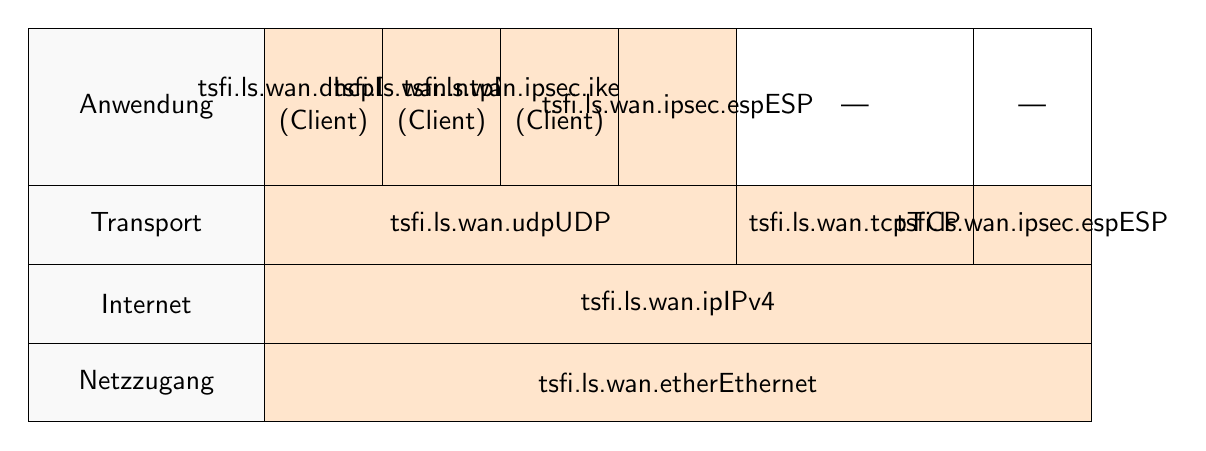
\begin{tikzpicture}
    [c/.style={midway,align=center,font=\sffamily},
      tsfi/.style={fill=orange!20},
      nontsf/.style={fill=yellow!20},
      none/.style={},      
      layer/.style={fill=gray!5}]

  \draw[layer] (0,0) rectangle ++(3,1) node[c]{Netzzugang};
  \draw[tsfi] (3,0) rectangle ++(10.5,1) node[c]{\hyperlink{tsfi.ls.wan.ether}{Ethernet}};

  \draw[layer] (0,1) rectangle ++(3,1) node[c]{Internet};
  \draw[tsfi] (3,1) rectangle ++(10.5,1) node[c]{\hyperlink{tsfi.ls.wan.ip}{IPv4}};

  \draw[layer] (0,2) rectangle ++(3,1) node[c]{Transport};
  \draw[tsfi] (3,2) rectangle ++(6,1) node[c]{\hyperlink{tsfi.ls.wan.udp}{UDP}};
  \draw[tsfi] (9,2) rectangle ++(3,1) node[c]{\hyperlink{tsfi.ls.wan.tcp}{TCP}};
  \draw[tsfi] (12,2) rectangle ++(1.5,1) node[c]{\hyperlink{tsfi.ls.wan.ipsec.esp}{ESP}};

  \draw[layer] (0,3) rectangle ++(3,2) node[c]{Anwendung};
  \draw[tsfi] (3,3) rectangle ++(1.5,2) node[c]{\hyperlink{tsfi.ls.wan.dhcp}{DHCP} \\ (Client)};
  \draw[tsfi] (4.5,3) rectangle ++(1.5,2) node[c]{\hyperlink{tsfi.ls.wan.ntp}{NTP} \\ (Client)};
  \draw[tsfi] (6,3) rectangle ++(1.5,2) node[c]{\hyperlink{tsfi.ls.wan.ipsec.ikev2}{IKEv2} \\ (Client)};
  \draw[tsfi] (7.5,3) rectangle ++(1.5,2) node[c]{\hyperlink{tsfi.ls.wan.ipsec.esp}{ESP}};
  \draw[none] (9,3) rectangle ++(3,2) node[c]{---};
  \draw[none] (12,3) rectangle ++(1.5,2) node[c]{---};

\end{tikzpicture}
  \caption{Protokolle auf \formatintf{LS.WAN} für die sicherheitsfunktionalen Anteile}
  \label{fig:tsfi.ls.wan.protocols}
\end{figure}


\hrefsubsection{tsfi.ls.wan.ether}{\tsfisectionname{ls.wan.ether}}

\sameprotocol{Ethernet}{WAN}{tsfi.ls.lan.ether}

\hrefsubsection{tsfi.ls.wan.ip}{\tsfisectionname{ls.wan.ip}}

\sameprotocol{IPv4 und ICMP}{WAN}{tsfi.ls.lan.ip}

\hrefsubsection{tsfi.ls.wan.tcp}{\tsfisectionname{ls.wan.tcp}}

\sameprotocol{TCP}{WAN}{tsfi.ls.lan.tcp}

\hrefsubsection{tsfi.ls.wan.udp}{\tsfisectionname{ls.wan.udp}}

\sameprotocol{UDP}{WAN}{tsfi.ls.lan.udp}

\hrefsubsection{tsfi.ls.wan.dhcp}{\tsfisectionname{ls.wan.dhcp}}

\tsfipurpose{tsfi.ls.wan.dhcp}

Der TOE bietet die Möglichkeit, auf der WAN-Schnittstelle als
DHCP-Client zu agieren. Der TOE kann also seine IP-Adresse von einem
DHCP-Server im WAN beziehen. Diese Funktion ist auf der Managementoberfläche
(de-)aktivierbar.

\calledsfmanual{ls.wan.dhcp}{\secfunclink{sf.networkservices}}

\tsfiparameters{tsfi.ls.wan.dhcp}

Das DHCP-Protokoll setzt auf dem UDP-Protokoll auf und ist in
\rfc[c]{2131} beschrieben. Die Beschreibungen enthalten
insbesondere das Format einer DHCP-Nachricht und die darin
enthaltenen Felder, die verschiedenen Nachrichtentypen und den Ablauf
der Kommunikation.

Das \rfc[c]{2132} dokumentiert zudem weitere DHCP-Optionen,
die der DHCP-Server mit dem DHCP-Client austauschen kann.

\hrefsubsection{tsfi.ls.wan.ntp}{\tsfisectionname{ls.wan.ntp}}

\tsfipurpose{tsfi.ls.wan.ntp}

Die Schnittstelle wird genutzt, um die Systemzeit mit Zeitservern aus dem
Internet zu synchronisieren. (\sfrlink{fpt_stm.1})

\calledsf{ls.wan.ntp}

\tsfiparameters{tsfi.ls.wan.ntp}

Die Protokollbeschreibung ist in \rfc[c]{5905}
dokumentiert. Der Zielport für den Client ist UDP-Port~123.

\hrefsubsection{tsfi.ls.wan.ipsec}{\tsfisectionname{ls.wan.ipsec}}

\tsfipurpose{tsfi.ls.wan.ipsec}

Der TOE verwendet die WAN-Schnittstelle für den Aufbau des VPN-Kanals Der TOE
bietet dafür IPsec als VPN-Client an der WAN-Schnittstelle an.

\calledsf{ls.wan.ipsec}

\tsfiparameters{tsfi.ls.wan.ipsec}

IPSec berücksichtigt die Vorgaben aus \rfc[c]{4301}. Der TOE verwendet
für IPSec zwei Protokolle. Zum Schlüsselaustausch wird das Protokoll
Internet Key Exchange (IKE) in der Version 2 nach \rfc[c]{7296}
am UDP-Port~500 verwendet. Für die Übertragung der Nutzdaten wird das
Encapsulation Security Payload (ESP) nach \rfc[c]{4303}
(IP-Protokollnummer 50, bzw. UDP-Port 4500) umgesetzt.

\hrefsubsubsection{tsfi.ls.wan.ipsec.ikev2}{Internet Key Exchange Version 2 (IKEv2)}

IKE selbst ist nicht für die Übertragung von Nutzdaten verantwortlich, sondern
lediglich für die Verteilung von geeignetem Schlüsselmaterial und die
Authentifizierung der zwei Parteien. Die Übertragung der eigentlichen Nutzdaten
ist die Aufgabe des ESP-Protokolls
(vgl. Abschnitt~\vref{tsfi.ls.wan.ipsec.esp}).

Der TOE als Initiator der VPN-Verbindungen schlägt zu Beginn des IKE-Protokolls
die zu verwendenden Algorithmen vor.


\hrefsubsubsection{tsfi.ls.wan.ipsec.esp}{Encrypted Security Payload (ESP)}

Das ESP-Protokoll gewährleistet Authentizität, Integrität und
Vertraulichkeit der übermittelten Daten. Dabei werden getrennte
Algorithmen für Verschlüsselung und Integritätssicherung verwendet.

Die in IKE für ESP ausgehandelte SA inklusive der benötigen Schlüssel
und Algorithmen wird nun verwendet, um die IP-Pakete, die über den
Tunnel verschickt werden sollen, zu sichern. Dazu wird die Struktur
des ESP-Headers verwendet, wie in
\figureref{fig:tsfi.ls.wan.ipsec.esp.header} dargestellt
(s.\,a. \cite[Figure~2]{rfc4303})


\begin{figure}[htbp]
  \centering
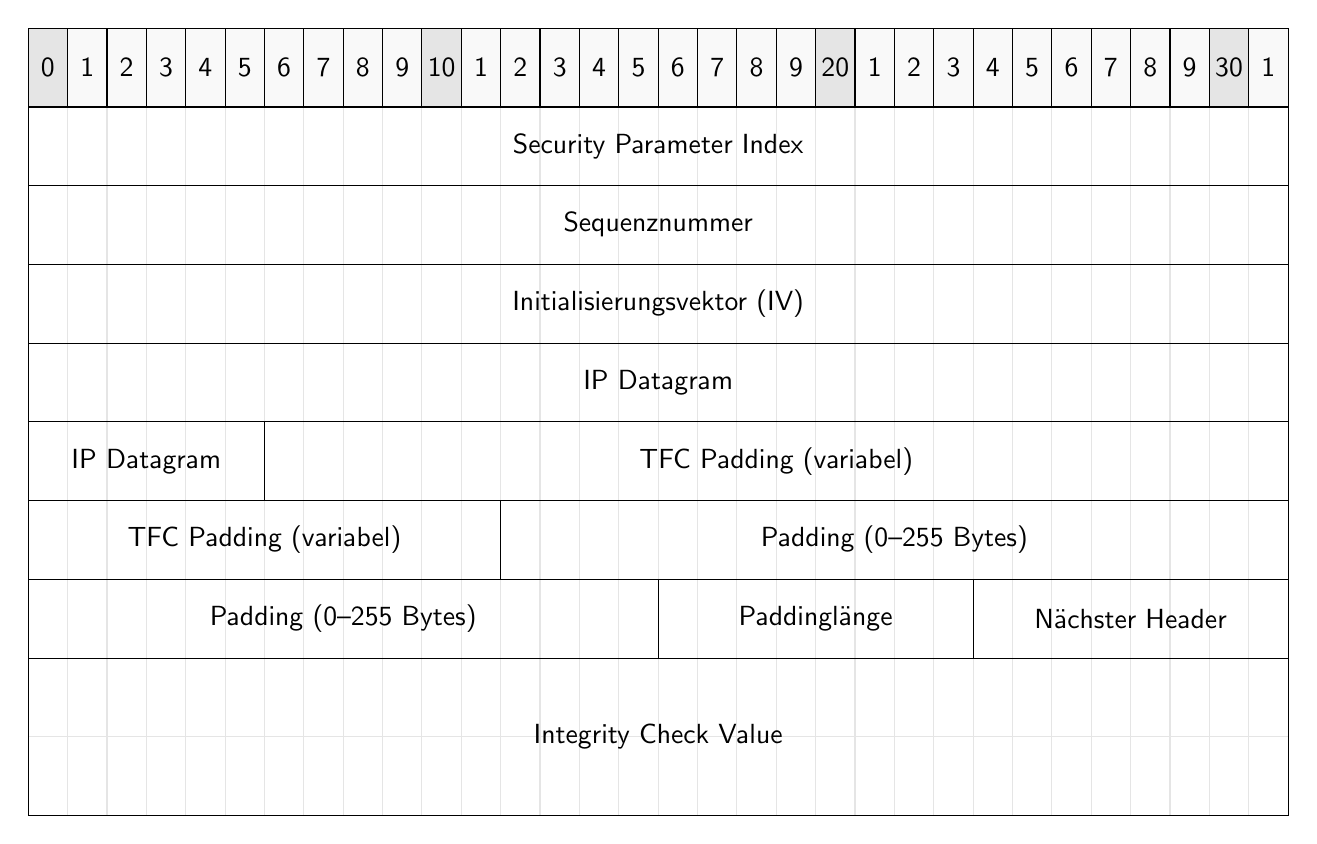
\begin{tikzpicture}
  [c/.style={midway,font=\sffamily},
  none/.style={},
  index/.style={fill=gray!5},
  index0/.style={fill=gray!20}]

  \draw[xstep=.5,gray!20, thin] (0,0) grid (16,9);

  \draw[index] (15.5,9) rectangle ++(0.5,1) node[c]{1};
  \draw[index0] (15,9) rectangle ++(0.5,1) node[c]{30};
  \draw[index] (14.5,9) rectangle ++(0.5,1) node[c]{9};
  \draw[index] (14,9) rectangle ++(0.5,1) node[c]{8};
  \draw[index] (13.5,9) rectangle ++(0.5,1) node[c]{7};
  \draw[index] (13,9) rectangle ++(0.5,1) node[c]{6};
  \draw[index] (12.5,9) rectangle ++(0.5,1) node[c]{5};
  \draw[index] (12,9) rectangle ++(0.5,1) node[c]{4};
  \draw[index] (11.5,9) rectangle ++(0.5,1) node[c]{3};
  \draw[index] (11,9) rectangle ++(0.5,1) node[c]{2};
  \draw[index] (10.5,9) rectangle ++(0.5,1) node[c]{1};
  \draw[index0] (10,9) rectangle ++(0.5,1) node[c]{20};
  \draw[index] (9.5,9) rectangle ++(0.5,1) node[c]{9};
  \draw[index] (9,9) rectangle ++(0.5,1) node[c]{8};
  \draw[index] (8.5,9) rectangle ++(0.5,1) node[c]{7};
  \draw[index] (8,9) rectangle ++(0.5,1) node[c]{6};
  \draw[index] (7.5,9) rectangle ++(0.5,1) node[c]{5};
  \draw[index] (7,9) rectangle ++(0.5,1) node[c]{4};
  \draw[index] (6.5,9) rectangle ++(0.5,1) node[c]{3};
  \draw[index] (6,9) rectangle ++(0.5,1) node[c]{2};
  \draw[index] (5.5,9) rectangle ++(0.5,1) node[c]{1};
  \draw[index0] (5,9) rectangle ++(0.5,1) node[c]{10};
  \draw[index] (4.5,9) rectangle ++(0.5,1) node[c]{9};
  \draw[index] (4,9) rectangle ++(0.5,1) node[c]{8};
  \draw[index] (3.5,9) rectangle ++(0.5,1) node[c]{7};
  \draw[index] (3,9) rectangle ++(0.5,1) node[c]{6};
  \draw[index] (2.5,9) rectangle ++(0.5,1) node[c]{5};
  \draw[index] (2,9) rectangle ++(0.5,1) node[c]{4};
  \draw[index] (1.5,9) rectangle ++(0.5,1) node[c]{3};
  \draw[index] (1,9) rectangle ++(0.5,1) node[c]{2};
  \draw[index] (0.5,9) rectangle ++(0.5,1) node[c]{1};
  \draw[index0] (0,9) rectangle ++(0.5,1) node[c]{0};

  \draw[none] (0,8) rectangle ++(16,1) node[c]{Security Parameter Index};

  \draw[none] (0,7) rectangle ++(16,1) node[c]{Sequenznummer};

  \draw[none] (0,6) rectangle ++(16,1) node[c]{Initialisierungsvektor (IV)};

  \draw[none] (0,5) rectangle ++(16,1) node[c]{IP Datagram};

  \draw[none] (3,4) rectangle ++(13,1) node[c]{TFC Padding (variabel)};
  \draw[none] (0,4) rectangle ++(3,1) node[c]{IP Datagram};

  \draw[none] (6,3) rectangle ++(10,1) node[c]{Padding~(0--255 Bytes)};
  \draw[none] (0,3) rectangle ++(6,1) node[c]{TFC Padding (variabel)};

  \draw[none] (12,2) rectangle ++(4,1) node[c]{Nächster Header};
  \draw[none] (8,2) rectangle ++(4,1) node[c]{Paddinglänge};
  \draw[none] (0,2) rectangle ++(8,1) node[c]{Padding~(0--255 Bytes)};

  \draw[none] (0,0) rectangle ++(16,2) node[c]{Integrity Check Value};

\end{tikzpicture}
  \caption{ESP Header}
  \label{fig:tsfi.ls.wan.ipsec.esp.header}
\end{figure}



% !TEX root = "../adv_fsp"
%%% Local Variables:
%%% mode: latex
%%% TeX-engine: luatex
%%% TeX-master: "../adv_fsp"
%%% TeX-parse-self: t
%%% TeX-auto-save: t
%%% End:
